%%%%%%%%%%%%%%%%%%%%%%%%%%%%%%%%%%%%%%%%%%%%%%%%%%%%%%%%%%%%%%%%%%%%%%
% Template-TA-Fisika-ITS.v.1.0 2022.01
%%%%%%%%%%%%%%%%%%%%%%%%%%%%%%%%%%%%%%%%%%%%%%%%%%%%%%%%%%%%%%%%%%%%%%
% oleh: 1. Sasfan Arman Wella, BRIN (sasfan.a.wella@gmail.com)
%       2. Nadya Amalia, BRIN (amalianadd@gmail.com)
%       3. Fitrotul Millah, ITS (fitrotulmillah2000@gmail.com)
%       4. Nathasya Veronica, ITS (nathasyaveronica363@gmail.com) 
%
%  NB: Template ini bukanlah template resmi dari ITS, namun disusun
%      berdasarkan pedoman penulisan laporan TA Fisika ITS
%
% [ Bila ada fitur yang ditambahkan dalam template ini, silahkan
%   tambahkan nama Anda setelah nama pembuat template sebelumnya ]
%
%  Penjelasan singkat dari template ini 
%  dapat dilihat pada file README
% 
%%%%%%%%%%%%%%%%%%%%%%%%%%%%%%%%%%%%%%%%%%%%%%%%%%%%%%%%%%%%%%%%%%%%%%

%=====================================================================
% FORMAT DAN PENGATURAN UMUM:
%=====================================================================
\documentclass[a5paper, 11pt, final, openright, twoside]{report}
%%%%%%%%%%%%%%%%%%%%%%%%%%%%%%%%%%%%%%%%%%%%%%%%%%%%%%%%%%%%%%%%%%%%%%
% FORMAT DAN PENGATURAN UMUM:
%=====================================================================
\usepackage{multirow}
\usepackage[table]{xcolor}
\usepackage{tabularx,tikz}
\usepackage{caption}
\usepackage{float}
\usepackage{listings}
\usepackage{subcaption}
\usepackage{graphicx}
\usepackage{enumitem}
\usepackage{amsmath,amssymb,charter,color}
\usepackage[hidelinks]{hyperref}
\usepackage[utf8]{inputenc}
\usepackage{lipsum} % hanya untuk membuat teks dummy
\usepackage{wrapfig}
\usepackage{emptypage}
\usepackage{setspace}
\usepackage{rotating}

%======================================================================
%   Mengatur margin 
%======================================================================
\usepackage[top=25mm,left=25mm,right=20mm,bottom=25mm]{geometry}
    \linespread{1.3} % Gunakan 1.3 untuk spasi satu setengah, 
                     % Gunakan 1.6 untukspasi dua
    
%======================================================================
%   Mengatur bahasa yang digunakan
%======================================================================

\usepackage[bahasa]{babel}
    \selectlanguage{bahasa}

%======================================================================
%   Mengatur format BAB, SUBBAB, Floating Gambar dan Tabel
%======================================================================

\usepackage[explicit]{titlesec}
    \titleformat{\chapter}[display]
        {\normalfont\bfseries\centering}
        {\large\MakeUppercase{\chaptername}~\thechapter}
        {0.5em}{\large \MakeUppercase{#1}}
    \titleformat{\section}
        {\normalfont\normalsize\bfseries}{\thesection}
        {0.5em}{#1}
    \titleformat{\subsection}
        {\normalfont\normalsize\bfseries}{\thesubsection}
        {0.5em}{#1}
    
\usepackage{tocloft,etoolbox}
\apptocmd{\appendix}
    {\addtocontents{toc}{  
    \protect\addtolength\protect\cftchapnumwidth{-\mylength}
    \protect\renewcommand{\protect\cftchappresnum}{LAMPIRAN~}
    \protect\settowidth\mylength{
    \bfseries\protect\cftchappresnum\protect\cftchapaftersnum}
    \protect\addtolength\protect\cftchapnumwidth{\mylength}}}{}{}
\newlength\mylength

\renewcommand\cftchappresnum{BAB~}
\settowidth\mylength{\bfseries\cftchappresnum\cftchapaftersnum}
\addtolength\cftchapnumwidth{\mylength}
\renewcommand{\cftdotsep}{1}
\renewcommand{\cftchapleader}{\cftdotfill{\cftsecdotsep}}

\renewcommand\cftfigpresnum{Gambar~}
\settowidth\mylength{\cftfigpresnum\cftfigaftersnum}
\addtolength\cftfignumwidth{\mylength}

\renewcommand\cfttabpresnum{Tabel~}
\settowidth\mylength{\cfttabpresnum\cfttabaftersnum}
\addtolength\cfttabnumwidth{\mylength}

%======================================================================
%   Mengatur background pada cover
%======================================================================
\usepackage[pages=some]{background}
\backgroundsetup{
    scale=1,
    color=black,
    opacity=1.0,
    angle=0,
    contents={%
    
\includegraphics[width=\paperwidth,height=\paperheight]
    {./halaman-depan/00-BGcover.jpg}
    }%
}

%======================================================================
%   Mengatur jenis font yang digunakan
%======================================================================
\usepackage{fontspec}
\setmainfont{Times New Roman} 
\setsansfont{Trebuchet MS} 
\setmonofont{Inconsolata}

%======================================================================
%   Untuk mendefinisikan halaman kosong
%======================================================================
\newcommand\halamanKosong{
    \newpage
    \vspace*{\fill}
    \begin{center}
        \textit{Halaman ini sengaja dikosongkan}
    \end{center}
    \vspace{\fill}
    \clearpage
}

%======================================================================
%   Mengatur agar paragraf pertama mempunyai indentasi
%======================================================================
\usepackage{indentfirst}
\setlength{\parindent}{2em} 

%======================================================================
%   Mengatur tentang jarak antara judul section dan paragraf
%======================================================================
\usepackage{titlesec}

\titlespacing\section{0pt}{12pt plus 4pt minus 2pt}{0pt plus 2pt minus 2pt}
\titlespacing\subsection{0pt}{12pt plus 4pt minus 2pt}{0pt plus 2pt minus 2pt}
\titlespacing\subsubsection{0pt}{12pt plus 4pt minus 2pt}{0pt plus 2pt minus 2pt}

%======================================================================
%   Mengatur header dan footer
%======================================================================
\usepackage{fancyhdr}
    \fancyhead{}
    \fancyfoot{}
    \setlength{\headheight}{15pt}
    \setlength{\headsep}{12pt}
    \setlength{\footskip}{30pt}
    \renewcommand{\headrulewidth}{0pt}
    \renewcommand{\footrulewidth}{0pt}
    
    \fancypagestyle{romawi}{%
    \setlength{\headheight}{15pt}
    \setlength{\headsep}{12pt}
    \setlength{\footskip}{30pt}
    \fancyfoot[CE,CO]{\thepage}
    \renewcommand{\headrulewidth}{0pt}
    \renewcommand{\footrulewidth}{0pt}
    }
    
    \fancypagestyle{konten}{%
    \setlength{\headheight}{15pt}
    \setlength{\headsep}{12pt}
    \setlength{\footskip}{30pt}
    \fancyhead[LE,RO]{\thepage}
    \fancyfoot[CE,CO]{}
    \renewcommand{\headrulewidth}{0pt}
    \renewcommand{\footrulewidth}{0pt}
    }
    
%======================================================================
%   Mengatur tentang format referensi
%======================================================================

\usepackage[square]{natbib}

%======================================================================
%   Mengatur template untuk menulis code
%======================================================================

\usepackage{listings}
\usepackage[framemethod=default]{mdframed}

\newmdenv[innerlinewidth=0.5pt, 
roundcorner=4pt,
linecolor=red,
innerleftmargin=6pt,
innerrightmargin=6pt,
innertopmargin=6pt,
innerbottommargin=6pt,
backgroundcolor=red,
]{mybox}
\newcommand{\unitcell}{\textit{unit cell }}
\newcommand{\exchange}{\textit{exchange }}
\newcommand{\corr}{\textit{correlation }}
\newcommand{\eh}[1]{{\color{red} EH:{#1}}}
\newcommand{\schro}{Schr{\"o}dinger }
\newcommand{\be}{\begin{equation}}
\newcommand{\ee}{\end{equation}}
\newcommand{\bea}{\begin{eqnarray}}
\newcommand{\eea}{\end{eqnarray}}
\newcommand{\HH}{{\cal H}}
\newcommand{\RR}{{\cal R}}
\newcommand{\p}{\partial}
\newcommand{\s}{\sigma}
\newcommand{\la}{\langle}
\newcommand{\ra}{\rangle}
\newcommand{\lla}{\left\langle}
\newcommand{\rra}{\right\rangle}
\newcommand{\lb}{\left[}
\newcommand{\rb}{\right]}
\newcommand{\lp}{\left(}
\newcommand{\rp}{\right)}
\newcommand{\Tr}{{\rm \, Tr\,}}
\newcommand{\bra}[1]{\la #1|}
\newcommand{\ket}[1]{| #1\ra}
\newcommand{\sgn}{{\rm sgn}\,}
\renewcommand{\Im}{{\rm Im}\,}
\renewcommand{\Re}{{\rm Re}\,}
\renewcommand{\vec}[1]{{\bf #1}}
\newcommand{\eps}{\varepsilon}
\renewcommand{\tilde}{\widetilde}
\def\nn{\nonumber\\}

\definecolor{codegreen}{rgb}{0,0.6,0}
\definecolor{codegray}{rgb}{0.5,0.5,0.5}
\definecolor{codepurple}{rgb}{0.58,0,0.82}
\definecolor{backcolour}{rgb}{0.95,0.95,0.92}

\lstdefinestyle{mystyle}{
    backgroundcolor=\color{backcolour},   
    commentstyle=\color{codegreen},
    keywordstyle=\color{magenta},
    numberstyle=\tiny\color{codegray},
    stringstyle=\color{codepurple},
    basicstyle=\ttfamily\small,
    breakatwhitespace=false,         
    breaklines=true,                 
    captionpos=b,                    
    keepspaces=true,                 
    numbers=left,                    
    numbersep=5pt,                  
    showspaces=false,                
    showstringspaces=false,
    showtabs=false,                  
    tabsize=2 
}

\lstset{style=mystyle}

%======================================================================
%   Agar sisi bagian kanan menjadi lebih rapih
%======================================================================
\emergencystretch=\maxdimen
\hyphenpenalty=10000
\hbadness=10000

%======================================================================
%   Mengatur jenis font untuk equations
%======================================================================
\usepackage{newtxmath}

%======================================================================
%   Mengatur format daftar isi, gambar, dan tabel
%======================================================================

\renewcommand{\cfttoctitlefont}{\hfil\large\bfseries\MakeUppercase}
\renewcommand{\cftloftitlefont}{\hfil\large\bfseries\MakeUppercase}
\renewcommand{\cftlottitlefont}{\hfil\large\bfseries\MakeUppercase}
\renewcommand{\cftsecleader}{\cftdotfill{\cftdotsep}}
\setlength\cftparskip{-2pt}
\setlength\cftbeforesecskip{2pt}
\setlength\cftbeforechapskip{2pt}

%%%%%%%%%%%%%%%%%%%%%%%%%%%%%%%%%%%%%%%%%%%%%%%%%%%%%%%%%%%%%%%%%%%%%%

%%%%%%%%%%%%%%%%%%%%%%%%%%%%%%%%%%%%%%%%%%%%%%%%%%%%%%%%%%%%%%%%%%%%%%
% TULISKAN INFORMASI-INFORMASI YANG DIBUTUHKAN DALAM DOKUMEN TUGAS AKHIR
%=====================================================================
% Judul Tugas Akhir
\newcommand{\kodeTA}{%
    TUGAS AKHIR -- TA 123456% Tuliskan kode mata kuliah dalam bahasa Indonesia
}
\newcommand{\kodeTAInggris}{%
    FINAL PROJECT -- TA 123456% Tuliskan kode mata kuliah dalam bahasa Inggris
} 
%=====================================================================
% Judul Tugas Akhir
\newcommand{\judulTA}{%
    Judul Tugas Akhir Mahasiswa/(i) dalam Bahasa Indonesia% Tuliskan judul dalam bahasa Indonesia
}
\newcommand{\judulTAInggris}{%
    Judul Tugas Akhir Mahasiswa/(i) dalam Bahasa Inggris% Tuliskan judul dalam bahasa Inggris
} 
%=====================================================================
% Nama Mahasiswa
\newcommand{\namaMahasiswa}{%
    Nama Lengkap% Tuliskan nama lengkap mahasiswa/(i)
} 
%=====================================================================
% Nomor Induk Mahasiswa
\newcommand{\noIndukMahasiswa}{%
    Nomor Induk Mahasiswa/(i)% Tuliskan nomor induk mahasiswa/(i)
}
%=====================================================================
% Email Mahasiswa
\newcommand{\emailMahasiswa}{%
    nama@email.com% Tuliskan alamat email mahasiswa/(i)
}
%=====================================================================
% Informasi Dosen Pembimbing 1
\newcommand{\namaDosenPembimbingSatu}{%
    Nama Pembimbing 1% Tuliskan nama Pembimbing 1
}
\newcommand{\nipDosenPembimbingSatu}{%
    NIP Pembimbing 1% Tuliskan NIP Pembimbing 1
}
%=====================================================================
% Informasi Dosen Pembimbing 2
\newcommand{\namaDosenPembimbingDua}{%
    Nama Pembimbing 2% Tuliskan nama Pembimbing 2
}
\newcommand{\nipDosenPembimbingDua}{%
    NIP Pembimbing 2% Tuliskan NIP Pembimbing 2
}
%=====================================================================
% Informasi Kepala Departemen
\newcommand{\namaKaDep}{%
    Nama Kepala Departemen% Tuliskan nama Kepala Departemen
}
\newcommand{\nipKaDep}{%
    NIP Kepala Departemen% Tuliskan NIP Kepala Departemen
}
%=====================================================================
% Informasi Kampus
%=====================================================================
\newcommand{\namaDepartemen}{%
    Departemen Fisika% Tuliskan nama Departemen dalam bahasa Indonesia
}
\newcommand{\namaDepartemenInggris}{%
    Department of Physics% Tuliskan nama Departemen dalam bahasa Inggris
}
\newcommand{\namaFakultas}{%
    Fakultas Sains dan Analitika Data% Tuliskan nama Fakultas dalam bahasa Indonesia
}
\newcommand{\namaFakultasInggris}{%
    Faculty of Science and Data Analytics% Tuliskan nama Fakultas dalam bahasa Inggris
}
\newcommand{\namaUniversitas}{%
    Institut Teknologi Sepuluh Nopember%
}
\newcommand{\namaKota}{%
    Surabaya%
}
%=====================================================================
%   Tanggal Pengesahan
%=====================================================================
\newcommand{\tanggalPengesahan}{%
    21 Januari 2022 % Tuliskan tanggal pengesahan Tugas Akhir
}
%%%%%%%%%%%%%%%%%%%%%%%%%%%%%%%%%%%%%%%%%%%%%%%%%%%%%%%%%%%%%%%%%%%%%%

%=====================================================================

%=====================================================================
% KODE RINGKAS UNTUK SIMBOL DAN SATUAN:
%=====================================================================
%%%%%%%%%%%%%%%%%%%%%%%%%%%%%%%%%%%%%%%%%%%%%%%%%%%%%%%%%%%%%%%%%%%%%%
% KODE RINGKAS UNTUK SIMBOL DAN SATUAN:
%=====================================================================
% Simbol Matematis
%---------------------------------------------------------------------

\def\imag{\mathrm{i}}
\def\euler{\mathrm{e}}
\def\diff{\mathrm{d}}

%---------------------------------------------------------------------
% Satuan
%---------------------------------------------------------------------

\def\unitangstrom{\,\textrm{\AA}}
\def\unitkg{\,\textrm{kg}}
\def\unitJ{\,\textrm{J}}
\def\unitev{\,\textrm{eV}}
\def\unitmev{\,\textrm{meV}}
\def\unitvolt{\,\textrm{V}}
\def\unitm{\,\textrm{m}}
\def\unitcm{\,\textrm{cm}}
\def\unitmm{\,\textrm{mm}}
\def\unitum{\,\mathrm{\mu}\textrm{m}}
\def\unitnm{\,\textrm{nm}}
\def\unitwn{\,\textrm{cm}^{-1}}
\def\unitsec{\,\textrm{s}}
\def\unitps{\,\textrm{ps}}
\def\unitfs{\,\textrm{fs}}
\def\unitdeg{^\circ}
\def\unitcelcius{\unitdeg\textrm{C}}
\def\unitpercent{\,\%}

%---------------------------------------------------------------------
% Singkatan
%---------------------------------------------------------------------

\def\its{\,Institut Teknologi Sepuluh Nopember}
\def\qe{\,\textsc{Quantum\:ESPRESSO}}
\def\btp{\,\textsc{BoltzTraP2}}
\def\schro{\,Schr\"{o}dinger}
\def\snse{\,SnSe}

%%%%%%%%%%%%%%%%%%%%%%%%%%%%%%%%%%%%%%%%%%%%%%%%%%%%%%%%%%%%%%%%%%%%%%


%=====================================================================


%=====================================================================
\begin{document}
%=====================================================================
    \pagestyle{romawi}
    \pagenumbering{roman}

    %======================================================================
%   Cover UTAMA
%======================================================================

    \thispagestyle{empty}

    \BgThispage
    
    \begin{flushleft}
        
\includegraphics[width=25mm]{./halaman-depan/00-Logo-ITS.png}
    \end{flushleft}
    
    \vspace{24mm}
    
    \noindent {\textsf{\color{white}{%
    \textbf{\kodeTA} % Nama dan kode mata kuliah
    }}}
    
    \vspace{4mm}
    
    \begin{flushleft}
        \noindent {\Large\textsf{\color{white}
        {\MakeUppercase{\textbf{\judulTA}}}}}
    \end{flushleft}
    
    \vspace{4mm}
    
    {\noindent\textsf{\color{white}
    {\MakeUppercase{\textbf{\namaMahasiswa}\\[-2mm]
    \textbf{NRP. \noIndukMahasiswa}}}}}
    
    \vspace{3mm}
    
    {\noindent\textsf{\color{white}{%
        \textbf{Dosen Pembimbing}\\[-2mm]
        \textbf{\namaDosenPembimbingSatu}\\[-2mm]
        \textbf{\namaDosenPembimbingDua}
    }}}
    
    \vspace{3mm}
    
    {\noindent\textsf{\color{white}{%
        \textbf{\namaDepartemen}\\[-2mm]
        \textbf{\namaFakultas}\\[-2mm]
        \textbf{\namaUniversitas}\\[-2mm]
        \textbf{\namaKota}\\[-2mm]
        \textbf{\the\year}
    }}}


%======================================================================
%   Menambahkan halaman kosong setelah cover utama
%======================================================================

\cleardoublepage

%======================================================================
%   Halaman judul (Bahasa Indonesia)
%======================================================================

{
\setcounter{page}{1}
\addcontentsline{toc}{chapter}{HALAMAN JUDUL}
    
\begin{flushleft}
    
\includegraphics[width=25mm]{./halaman-depan/00-Logo-ITS.png}
\end{flushleft}
    
\vspace{24mm}
    
\noindent {\textsf{\color{black}{%
\textbf{\kodeTA} % Nama dan kode mata kuliah
}}}
    
\vspace{4mm}
    
\begin{flushleft}
    \noindent {\Large\textsf{\color{black}
    {\MakeUppercase{\textbf{\judulTA}}}}}
\end{flushleft}
    
\vspace{4mm}
    
{\noindent\textsf{\color{black}
{\MakeUppercase{\textbf{\namaMahasiswa}\\[-2mm]
\textbf{NRP. \noIndukMahasiswa}}}}}
    
\vspace{3mm}
    
{\noindent\textsf{\color{black}{%
    \textbf{Dosen Pembimbing}\\[-2mm]
    \textbf{\namaDosenPembimbingSatu}\\[-2mm]
    \textbf{\namaDosenPembimbingDua}
}}}
    
\vspace{3mm}
    
{\noindent\textsf{\color{black}{%
    \textbf{\namaDepartemen}\\[-2mm]
    \textbf{\namaFakultas}\\[-2mm]
    \textbf{\namaUniversitas}\\[-2mm]
    \textbf{\namaKota}\\[-2mm]
    \textbf{\the\year}
}}}

%======================================================================
%   Mengambahkan halaman kosong setelah cover utama
%======================================================================

\halamanKosong

%======================================================================
%   Halaman judul (Bahasa Inggris)
%======================================================================

\begin{flushleft}
    
\includegraphics[width=25mm]{./halaman-depan/00-Logo-ITS.png}
\end{flushleft}
    
\vspace{24mm}
    
\noindent {\textsf{\color{black}{%
\textbf{\kodeTAInggris} % Nama dan kode mata kuliah dalam bahasa Inggris
}}}
    
\vspace{4mm}
    
\begin{flushleft}
    \noindent {\Large\textsf{\color{black}
    {\MakeUppercase{\textbf{\judulTAInggris}}}}}
\end{flushleft}
    
\vspace{4mm}
    
{\noindent\textsf{\color{black}
{\MakeUppercase{\textbf{\namaMahasiswa}\\[-2mm]
\textbf{NRP. \noIndukMahasiswa}}}}}
    
\vspace{3mm}
    
{\noindent\textsf{\color{black}{%
    \textbf{Dosen Pembimbing}\\[-2mm]
    \textbf{\namaDosenPembimbingSatu}\\[-2mm]
    \textbf{\namaDosenPembimbingDua}
}}}
    
\vspace{3mm}
    
{\noindent\textsf{\color{black}{%
    \textbf{\namaDepartemenInggris}\\[-2mm]
    \textbf{\namaFakultasInggris}\\[-2mm]
    \textbf{\namaUniversitas}\\[-2mm]
    \textbf{\namaKota}\\[-2mm]
    \textbf{\the\year}
}}}

}
    \halamanKosong
    
%---------------------------------------------------------------------
%    HALAMAN DEPAN
%---------------------------------------------------------------------
    
    % LEMBAR PENGESAHAN
    %%%%%%%%%%%%%%%%%%%%%%%%%%%%%%%%%%%%%%%%%%%%%%%%%%%%%%%%%%%%%%%%%%%%%%
%
%   Secara umum, informasi yang dibutuhkan pada lembar pengesahan
%   ini diambil dari file "informasi.tex"
%
%%%%%%%%%%%%%%%%%%%%%%%%%%%%%%%%%%%%%%%%%%%%%%%%%%%%%%%%%%%%%%%%%%%%%%

\begin{center}
    {\large\textbf{LEMBAR PENGESAHAN}}
    \addcontentsline{toc}{chapter}{LEMBAR PENGESAHAN}
    \pagestyle{fancy}
\end{center}

%---------------------------------------------------------------------

\begin{center}
    
    {\large\MakeUppercase{\textbf{{\judulTA}}}}

    \vspace{5mm}
        
    {\large\textbf{TUGAS AKHIR}}

    \vspace{2mm}
    
    Diajukan untuk memenuhi syarat dalam \\[-2mm] 
    memperoleh gelar sarjana pada: \\[-2mm]
    %
    Program Sarjana \namaDepartemen \\[-2mm]
    \namaFakultas \\[-2mm]
    \namaUniversitas \\[-2mm]
    \namaKota \\[-2mm]

    \vspace{6mm}
    
    Oleh: \\
    
    {\textbf{\MakeUppercase{\namaMahasiswa}}}\\
    {\textbf{\MakeUppercase{\noIndukMahasiswa}}}\\

\end{center}

%---------------------------------------------------------------------

\begin{flushleft}
Disetujui oleh Dosen Pembimbing Tugas Akhir \\[2mm]

\begin{tabular}{ l c l c}
    Pembimbing I    & : & \namaDosenPembimbingSatu &
    ($\quad\quad\quad$) \\
                    &   & NIP. \nipDosenPembimbingSatu  & \\
    Pembimbing II   & : & \namaDosenPembimbingDua  &
    ($\quad\quad\quad$) \\
                    &   & NIP. \nipDosenPembimbingDua  & \\
\end{tabular}
\end{flushleft}

\vfill

\begin{flushright}
    \namaKota, \tanggalPengesahan
\end{flushright}

\vfill

%%%%%%%%%%%%%%%%%%%%%%%%%%%%%%%%%%%%%%%%%%%%%%%%%%%%%%%%%%%%%%%%%%%%%%
    \halamanKosong

    % ABSTRAK
    %%%%%%%%%%%%%%%%%%%%%%%%%%%%%%%%%%%%%%%%%%%%%%%%%%%%%%%%%%%%%%%%%%%%%%
%
%   Abstrak
%
%%%%%%%%%%%%%%%%%%%%%%%%%%%%%%%%%%%%%%%%%%%%%%%%%%%%%%%%%%%%%%%%%%%%%%

\begin{center}
    \addcontentsline{toc}{chapter}{ABSTRAK}
    \pagestyle{fancy}
\end{center}

%---------------------------------------------------------------------

\begin{center}
    {\textbf{\MakeUppercase{\judulTA}}}
\end{center}

\vspace{5mm}

\noindent \begin{tabular}{l c l}
    \textbf{Nama}       & \textbf{:} & \textbf{\namaMahasiswa}  \\[-1mm]
    \textbf{NRP}        & \textbf{:} & \textbf{\noIndukMahasiswa}  \\[-1mm]
    \textbf{Departemen} & \textbf{:} & \textbf{\namaDepartemen}  \\[-1mm]
    \textbf{Pembimbing} & \textbf{:} & \textbf{1. \namaDosenPembimbingSatu}  \\[-1mm]
                        &            & \textbf{2. \namaDosenPembimbingDua}
\end{tabular}

%---------------------------------------------------------------------

\vspace{5mm}

\begin{center}
    \noindent {\textbf{{Abstrak}}}
\end{center}

%---------------------------------------------------------------------

% Catatan: Gunakan \singlespacing di tiap awal paragraf

{\singlespacing\indent%
Ini adalah contoh dokumen Tugas Akhir yang dibuat dengan menggunakan \textit{template} \LaTeX{} dengan format yang telah disesuaikan dengan aturan penulisan Tugas Akhir yang berlaku di Departemen Fisika, \its{} (ITS). \textit{Template} ini dibuat dengan tujuan untuk memudahkan mahasiswa/(i) dalam melakukan penyusunan Tugas Akhir sekaligus untuk dapat digunakan sebagai \textit{template} yang berlaku umum, dengan beberapa penyesuaian untuk Tugas Akhir di Departemen lain di ITS. \textit{File} Tugas Akhir dalam format \texttt{$^*$.pdf} akan dapat dihasilkan dengan mengkompilasi \texttt{main.tex} menggunakan \textit{compiler} Lua\LaTeX.
}

%---------------------------------------------------------------------

\vspace{5mm}

\noindent \textbf{Kata kunci:} \textit{katakunci-1, katakunci-2, katakunci-3, katakunci-4} % Kata kunci dalam bahasa Indonesia

%%%%%%%%%%%%%%%%%%%%%%%%%%%%%%%%%%%%%%%%%%%%%%%%%%%%%%%%%%%%%%%%%%%%%%
    \halamanKosong
    
    %%%%%%%%%%%%%%%%%%%%%%%%%%%%%%%%%%%%%%%%%%%%%%%%%%%%%%%%%%%%%%%%%%%%%%
%
%   Abstract
%
%%%%%%%%%%%%%%%%%%%%%%%%%%%%%%%%%%%%%%%%%%%%%%%%%%%%%%%%%%%%%%%%%%%%%%

\begin{center}
    \addcontentsline{toc}{chapter}{\textit{ABSTRACT}}
    \pagestyle{fancy}
\end{center}

%---------------------------------------------------------------------

\begin{center}
    {\textbf{\MakeUppercase{\judulTAInggris}}}
\end{center}

\vspace{5mm}

\noindent \begin{tabular}{l c l}
    \textbf{Name}       & \textbf{:} & \textbf{\namaMahasiswa}  \\[-1mm]
    \textbf{NRP}        & \textbf{:} & \textbf{\noIndukMahasiswa}  \\[-1mm]
    \textbf{Department} & \textbf{:} & \textbf{\namaDepartemenInggris}  \\[-1mm]
    \textbf{Supervisors}& \textbf{:} & \textbf{1. \namaDosenPembimbingSatu}  \\[-1mm]
                        &            & \textbf{2. \namaDosenPembimbingDua}
\end{tabular}

%---------------------------------------------------------------------

\vspace{5mm}

\begin{center}
    \noindent {\textbf{{\textit{Abstract}}}}
\end{center}

%---------------------------------------------------------------------

% Catatan: Gunakan \singlespacing di tiap awal paragraf

{\singlespacing\indent% 
Abstrak Tugas Akhir dalam bahasa Inggris dituliskan di sini.
}

%---------------------------------------------------------------------

\vspace{5mm}

\noindent \textbf{Keywords:} \textit{katakunci-1, katakunci-2, katakunci-3, katakunci-4} % Kata kunci dalam bahasa Inggris

%%%%%%%%%%%%%%%%%%%%%%%%%%%%%%%%%%%%%%%%%%%%%%%%%%%%%%%%%%%%%%%%%%%%%%
    \halamanKosong
    
    % KATA PENGANTAR 
    %%%%%%%%%%%%%%%%%%%%%%%%%%%%%%%%%%%%%%%%%%%%%%%%%%%%%%%%%%%%%%%%%%%%%%

\begin{center}
    {\textbf{KATA PENGANTAR}}
    \addcontentsline{toc}{chapter}{KATA PENGANTAR}
    \pagestyle{fancy}
\end{center}

Kata pengantar untuk Tugas Akhir yang berjudul “{\MakeUppercase{\textbf{\judulTA}}}”, untuk memenuhi persyaratan menyelesaikan pendidikan strata satu (S1) di \namaDepartemen, \namaFakultas, \namaUniversitas. Ucapan terima kasih kepada berbagai pihak dapat diungkapkan pada bagian ini. 

\vspace{6mm}

\begin{flushright}

\namaKota, \tanggalPengesahan

\vspace{6mm}

Penulis

\end{flushright}

\newpage
    %\halamanKosong 

    % DAFTAR ISI  
        \addcontentsline{toc}{chapter}{DAFTAR ISI}
    \tableofcontents
    \newpage
    %\halamanKosong 
    
    % DAFTAR GAMBAR
        \addcontentsline{toc}{chapter}{DAFTAR GAMBAR}
    \listoffigures
    \newpage
    %\halamanKosong
    
    % DAFTAR TABEL
        \addcontentsline{toc}{chapter}{DAFTAR TABEL}
    \listoftables
    \newpage
    %\halamanKosong
    
%---------------------------------------------------------------------
%   KONTEN
%   Silahkan buat file bab isian di folder "konten"
%---------------------------------------------------------------------

    %%%%%%%%%%%%%%%%%%%%%%%%%%%%%%%%%%%%%%%%%%%%%%%%%%%%%%%%%%%%%%%%%%%%%%
% BAB PENDAHULUAN:
%=====================================================================
\pagenumbering{arabic}
\renewcommand{\thechapter}{\Roman{chapter}}
\addtocontents{toc}{\vskip10pt}
\chapter{PENDAHULUAN}
\renewcommand{\thechapter}{\arabic{chapter}}
\pagestyle{konten}
%---------------------------------------------------------------------

%=====================================================================
\section{Latar Belakang}
%=====================================================================

\textit{Template} \LaTeX{} untuk Tugas Akhir ini terdiri dari beberapa bagian, di mana \textit{file} \texttt{main.tex} merupakan bagian utama yang berguna untuk menyatakan dan mengatur kerangka serta \textit{input} yang digunakan dalam dokumen Tugas Akhir. \textit{File} Tugas Akhir dalam format \texttt{$^*$.pdf} akan dapat dihasilkan dengan mengkompilasi \texttt{main.tex} menggunakan \textit{compiler} Lua\LaTeX. Selain itu, bagian lain yang juga penting dan dapat diubah adalah:

\setlist{nolistsep}
\begin{enumerate}[noitemsep]
    %
    \item \textit{File} \texttt{informasi.tex}, untuk memuat informasi seperti nama mahasiswa/(i), nomor induk mahasiswa, nama dosen pembimbing, NIP dosen pembimbing, nama dosen penguji, NIP dosen penguji, nama kepala departemen, NIP kepala departemen, nama departemen hingga nama perguruan tinggi, dan tanggal pengesahan Tugas Akhir.
    %
    \item \textit{Folder} \texttt{gambar}, berisi \textit{file} gambar dengan format \texttt{jpg}, \texttt{jpeg}, \texttt{png}, \texttt{pdf}, \texttt{tiff} dan/atau \texttt{eps} yang akan dimuat dalam dokumen Tugas Akhir.
    %
    \item \textit{Folder} \texttt{halaman-depan}, berisi \textit{file} \texttt{$^*$.tex} dan gambar yang akan dimuat di bagian depan, sebelum bab Pendahuluan, dokumen Tugas Akhir. Abstrak dalam bahasa Indonesia dituliskan dalam \textit{file} \texttt{abstrak.tex}, sementara abstrak dalam bahasa Inggris dituliskan dalam \textit{file} \texttt{abstract.tex}.
    %
    \item \textit{File} \texttt{kodeUnit.tex}, untuk memuat kode ringkas dari simbol, satuan, dan singkatan yang digunakan dalam dokumen Tugas Akhir.
    %
    \item \textit{Folder} \texttt{konten}, berisi \textit{file} \texttt{$^*$.tex} dari bagian-bagian yang akan dimasukkan ke dalam Tugas Akhir, dari bab Pendahuluan hingga Penutup.
    %
    \item \textit{File} \texttt{pustaka.bib}, merupakan \textit{file} BibTeX yang berisi daftar referensi yang digunakan dalam dokumen Tugas Akhir.
    %
    \item \textit{Folder} \texttt{halaman-belakang}, berisi \textit{file} \texttt{biografi.tex} untuk memuat biografi singkat mahasiswa/(i) dan \textit{folder} \texttt{lmapiran} yang berisi \textit{file} \texttt{$^*$.tex} untuk memuat lampiran.
\end{enumerate}


%=====================================================================
\section{Rumusan Masalah}
%=====================================================================

Format pengetikan pada \textit{template} \LaTeX{} Tugas Akhir ini telah menyesuaikan dengan ketentuan yang berlaku di Departemen Fisika, \its{} (ITS). Di antaranya, jenis dan ukuran kertas, jarak spasi, jarak tepi (\textit{margin}), dan jenis huruf. Sehingga, mahasiswa/(i) dapat fokus kepada isi dan substansi dari Tugas Akhir yang disusun.



%=====================================================================
\section{Tujuan}
%=====================================================================

%Lorem ipsum.
%\setlist{nolistsep}
%\begin{enumerate}[noitemsep]
%    \item Lorem ipsum.
%    \item ...
%\end{enumerate}


%===================================================================
\section{Batasan Masalah}
%===================================================================

%Lorem ipsum.
%\setlist{nolistsep}
%\begin{enumerate}[noitemsep]
%    \item Lorem ipsum.
%    \item ...
%\end{enumerate}


%=====================================================================
\section{Manfaat}
%=====================================================================

%Lorem ipsum.
%\setlist{nolistsep}
%\begin{enumerate}[noitemsep]
%    \item Lorem ipsum.
%    \item ...
%\end{enumerate}


%=====================================================================
\section{Sistematika Penulisan}
%=====================================================================

\vspace{3mm}

% CATATAN: Bila diperlukan, sistematika penulisan ini dapat dipisah menjadi
% dua bagian agar bisa terpisah menjadi dua halaman.

\begin{tabular}{ p{0.15\textwidth} p{0.05\textwidth} p{0.60\textwidth}}
    \textbf{BAB I}  & \textbf{:} &
    \textbf{PENDAHULUAN} \\
    && 
    Tuliskan paparan singkat mengenai isi bagian Pendahuluan di sini \\ 
    %
    \textbf{BAB II}  & \textbf{:} &
    \textbf{TINJAUAN PUSTAKA} \\
    &&
    Tuliskan paparan singkat mengenai isi bagian Tinjauan Pustaka di sini \\
    % 
    \textbf{BAB III}  & \textbf{:} &
    \textbf{METODOLOGI} \\
    && 
    Tuliskan paparan singkat mengenai isi bagian Metodologi di sini \\ 
    % 
    \textbf{BAB IV} & \textbf{:} &
    \textbf{ANALISIS DAN PEMBAHASAN} \\
    && 
    Tuliskan paparan singkat mengenai isi bagian Analisis dan Pembahasan di sini \\
    %
    \textbf{BAB V} & \textbf{:} &
    \textbf{PENUTUP} \\
    && 
    Tuliskan paparan singkat mengenai isi bagian Penutup di sini \\
    %
    \multicolumn{3}{l}{\textbf{LAMPIRAN}}\\
    &&
    Tuliskan paparan singkat mengenai isi bagian Lampiran di sini \\
    %
\end{tabular}

%%%%%%%%%%%%%%%%%%%%%%%%%%%%%%%%%%%%%%%%%%%%%%%%%%%%%%%%%%%%%%%%%%%%%%
    %%%%%%%%%%%%%%%%%%%%%%%%%%%%%%%%%%%%%%%%%%%%%%%%%%%%%%%%%%%%%%%%%%%%%%
% BAB TINJAUAN PUSTAKA
%=====================================================================
\renewcommand{\thechapter}{\Roman{chapter}}
\addtocontents{toc}{\vskip10pt}
\chapter{TINJAUAN PUSTAKA}
\renewcommand{\thechapter}{\arabic{chapter}}
%---------------------------------------------------------------------

%=====================================================================
\section{Melakukan Sitasi }
%=====================================================================

Referensi berupa artikel dari jurnal ilmiah yang digunakan dalam dokumen Tugas Akhir ini, dan datanya telah dimasukkan dalam \texttt{pustaka.bib}, dapat disitasi dengan cara \citet{refJurnal} atau \citep{refJurnal}. Referensi yang digunakan juga dapat berupa artikel dari \textit{proceedings} ilmiah dan buku \citep{refProceedings,refBuku}. Referensi berupa laman internet dapat langsung dituliskan sebagai \url{https://phys.org/news/2021-11-thermoelectric-crystal-high.html} atau dengan melakukan sitasi \citep{refInternet}.

%=====================================================================
\section{Menuliskan Persamaan Matematika}
%=====================================================================

Suatu persamaan dapat dituliskan seperti contoh persamaan \textit{figure of merit} termoelektrik berikut:

\begin{equation}
    ZT = \dfrac{S^2 \sigma}{\kappa} T,
    \label{eq:persamaan1}
\end{equation}

\noindent di mana, $S$ adalah koefisien Seebeck dengan satuan V.K$^{-1}$, $\sigma$ adalah konduktivitas listrik dengan satuan S/m, $\kappa$ adalah konduktivitas panas dengan satuan W.m$^{-1}$.K$^{-1}$, dan $T$ adalah suhu termoelektrik dengan satuan K. 

Persamaan~\ref{eq:persamaan1} adalah contoh persamaan matematika dengan penomoran. Nomor persamaan pada \textit{template} \LaTeX{} Tugas Akhir ini telah diatur untuk diurutkan berdasarkan urutan kemunculan (posisi) persamaan tersebut dalam \textit{file} \texttt{$^*$.tex} dalam bagian \texttt{konten}. Untuk menuliskan persamaan tanpa penomoran dapat digunakan:

\begin{displaymath}
    \kappa = \kappa_{\rm e} + \kappa_{\rm l}
\end{displaymath}

\noindent Berbeda dengan Persamaan~\ref{eq:persamaan1}, persamaan di atas tidak memiliki nomor.


%=====================================================================
\section{Membuat Tabel}
%=====================================================================

Pada dasarnya ada berbagai tipe tabel. Tabel~\ref{tab:tabel1} adalah contoh tabel yang paling umum digunakan, yang terdiri atas 3 kolom dan 4 baris.

\begin{table}[ht] % [h] menyatakan posisi. h: here, t: top, b: bottom
	\centering
	\caption{Contoh tabel yang paling umum digunakan}
	\label{tab:tabel1}
	\begin{tabular}{c c c} % c: center, l: left (rata kiri), r: right (rata kanan)
		\hline
		Kolom-1 baris-1   & Kolom-2 baris-1   & Kolom-3 baris-1 \\
		\hline
		Kolom-1 baris-2   & Kolom-2 baris-2   & Kolom-3 baris-2 \\
		Kolom-1 baris-3   & Kolom-2 baris-3   & Kolom-3 baris-3 \\
		Kolom-1 baris-4   & Kolom-2 baris-4   & Kolom-3 baris-4 \\
		\hline
	\end{tabular}
\end{table}

\begin{sidewaystable}[h!] % [h] menyatakan posisi. h: here, t: top, b: bottom
	\centering
	\caption{Contoh tabel dengan \textit{multicolumn} dan \textit{multirow}}
	\label{tab:multitab}
	\begin{tabular}{l c c r} % c: center, l: left (rata kiri), r: right (rata kanan)
		\hline
		\multirow{2}{*}{Kol-1 baris-1/2}  & \multicolumn{2}{c}{Kol-2/3 baris 1}  & \multirow{2}{*}{Kol-4 baris-1/2} \\
		                                  & Kol-2 baris-2                        & Kol-3 baris-2   & \\
		\hline
		Kol-1 baris-3  & Kol-2 baris-3    & Kol-3 baris-3   & Kol-4 baris-3 \\
		Kol-1 baris-4  & Kol-2 baris-4    & Kol-3 baris-4   & \multirow{2}{*}{Kol-4 baris-4/5} \\
		Kol-1 baris-5  & $^*$Kol-2 baris-5    & $^{**}$Kol-3 baris-5   & \\		                                  
		\hline
		\multicolumn{4}{r}{$^*$\citealt{refJurnal}} \\ % Contoh sitasi catatan kaki
		\multicolumn{4}{r}{$^{**}$\citealt{refProceedings}} % Contoh sitasi catatan kaki
	\end{tabular}
\end{sidewaystable}

Sementara itu, Tabel~\ref{tab:multitab} adalah contoh tabel \textit{landscape} yang menggunakan \textit{multicolumn} dan \textit{multirow}, yang pada dasarnya terdiri dari 4 kolom dan 5 baris.

\newpage % Untuk melanjutkan bagian di bawah ini pada halaman baru
%---------------------------------------------------------------------
\subsection{Memasukkan Gambar dan Kode}
%---------------------------------------------------------------------

\textit{File} gambar perlu diunggah terlebih dahulu ke dalam folder \texttt{gambar}. Keterangan Gambar~\ref{fig:gambar1} dapat dituliskan pada \texttt{caption}.

\begin{figure}[h] % [h] menyatakan posisi. h: here, t: top, b: bottom
    \centering
    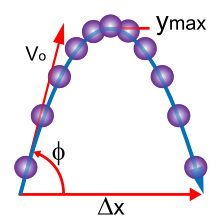
\includegraphics[width=5cm]{./gambar/contoh.png}
    \caption{Keterangan gambar dapat dituliskan di sini.}
    \label{fig:gambar1}
\end{figure}

Apabila mahasiswa/(i) perlu untuk menampilkan kode, \textit{script} program atau sejenisnya, contoh di bawah ini dapat digunakan sebagai acuan.

{\color{blue}
\begin{lstlisting}
sudo apt install build-essential g++ gfortran 
sudo apt install libblas-dev liblapack-dev 
    libopenmpi-dev libscalapack-mpi-dev 
\end{lstlisting}
}


%---------------------------------------------------------------------
\subsection{Memuat kode ringkas dari simbol, satuan, dan singkatan}
%---------------------------------------------------------------------

Untuk memuat kode ringkas dari simbol, satuan, dan singkatan yang telah dinyatakan dalam \texttt{kodeUnit.tex}, sebagai contoh, dapat dilakukan dengan \schro{} atau \its. Kode tersebut dapat diubah dan kode lain dapat ditambahkan pada \texttt{kodeUnit.tex}.

\newpage
%---------------------------------------------------------------------
\subsection{Daftar kode untuk simbol matematika dan Yunani}
%---------------------------------------------------------------------

\begin{tabular}{l l}
$\leq$ &  $\backslash$leq \\
$\geq$ &  $\backslash$geq \\
$\neq$ &  $\backslash$neq \\
$\nleq$ &  $\backslash$nleq \\
$\ngeq$ &  $\backslash$ngeq \\
$\cong$ &  $\backslash$cong \\
$\equiv$ &  $\backslash$equiv \\
$\sim$ &  $\backslash$sim \\
$\approx$ &  $\backslash$approx \\
$\times$ &  $\backslash$times \\
$\cdot $ &  $\backslash$cdot \\
$\ast $ &  $\backslash$ast \\
$\div$ &  $\backslash$div \\
$\pm$ &  $\backslash$pm \\
$\mp$ &  $\backslash$mp \\
$\oplus$ &  $\backslash$oplus \\
$\otimes$ &  $\backslash$otimes \\
$\propto $ &  $\backslash$propto \\
$\infty$ & $\backslash$infty \\
$\because$ &  $\backslash$because \\
$\therefore$ &  $\backslash$therefore \\
\end{tabular}
\hspace*{1ex}
\begin{tabular}{ll}
$\in$ &  $\backslash$in \\
$\subset $ &  $\backslash$subset \\
$\subseteq $ &  $\backslash$subseteq \\
$\varnothing $ &  $\backslash$varnothing  \\
$\cap $ &  $\backslash$cap \\
$\cup $ &  $\backslash$cup \\
$\Rightarrow$ &  $\backslash$Rightarrow \\
$\rightarrow$ &  $\backslash$rightarrow \\
$\partial$ &  $\backslash$partial \\
$90^\circ$ &  90$^\wedge\backslash$circ \\
$\parallel$ &  $\backslash$parallel \\
$\bot$ &  $\backslash$bot \\
$\triangle$ &  $\backslash$triangle \\
$\nabla$ &   $\backslash$nabla \\
$\angle$ &  $\backslash$angle \\
$\Pi$ &  $\backslash$Pi \\
$\Theta$ &  $\backslash$Theta \\
$\Gamma$ &  $\backslash$Gamma \\
$\Delta$ &  $\backslash$Delta \\
$\Omega$ &  $\backslash$Omega \\
$\Sigma$ &  $\backslash$Sigma \\
\end{tabular}
\hspace*{1ex}
\begin{tabular}{l l}
\& & $\backslash$\& \\
\% & $\backslash$\% \\
$\alpha$ &  $\backslash$alpha \\
$\beta$ &  $\backslash$beta \\
$\epsilon$ &  $\backslash$epsilon \\
$\zeta$ &  $\backslash$zeta \\
$\eta$ &  $\backslash$eta \\
$\kappa$ &  $\backslash$kappa \\
$\lambda$ &  $\backslash$lambda \\
$\mu$ &  $\backslash$mu \\
$\xi$ &  $\backslash$xi \\
$\rho$ &  $\backslash$rho \\
$\tau$ &  $\backslash$tau \\
$\phi$ &  $\backslash$phi \\
$\psi$ &  $\backslash$psi \\
$\pi$ &  $\backslash$pi \\
$\theta$ &  $\backslash$theta \\
$\gamma$ &  $\backslash$gamma\\
$\delta$ &  $\backslash$delta \\
$\omega$ &  $\backslash$omega \\
$\sigma$ &  $\backslash$sigma \\
\end{tabular}
 

\newpage

    %%%%%%%%%%%%%%%%%%%%%%%%%%%%%%%%%%%%%%%%%%%%%%%%%%%%%%%%%%%%%%%%%%%%%%
% BAB METODOLOGI
%=====================================================================
\renewcommand{\thechapter}{\Roman{chapter}}
\addtocontents{toc}{\vskip10pt}
\chapter{METODOLOGI}
\renewcommand{\thechapter}{\arabic{chapter}}
%---------------------------------------------------------------------

%=====================================================================
\section{Diagram Alir Penelitian}
%=====================================================================

Dalam penelitian, untuk diperoleh hasil yang baik maka dalam melakukan penelitian harus melalui tahapan-tahapan secara urut dan runtut. Tahapan-tahapan tersebut digambarkan dalam bentuk diagram alir yang ditunjukkan pada Gambar~\ref{fig:diagramAlirPenelitian}.

\begin{figure}
    \centering
    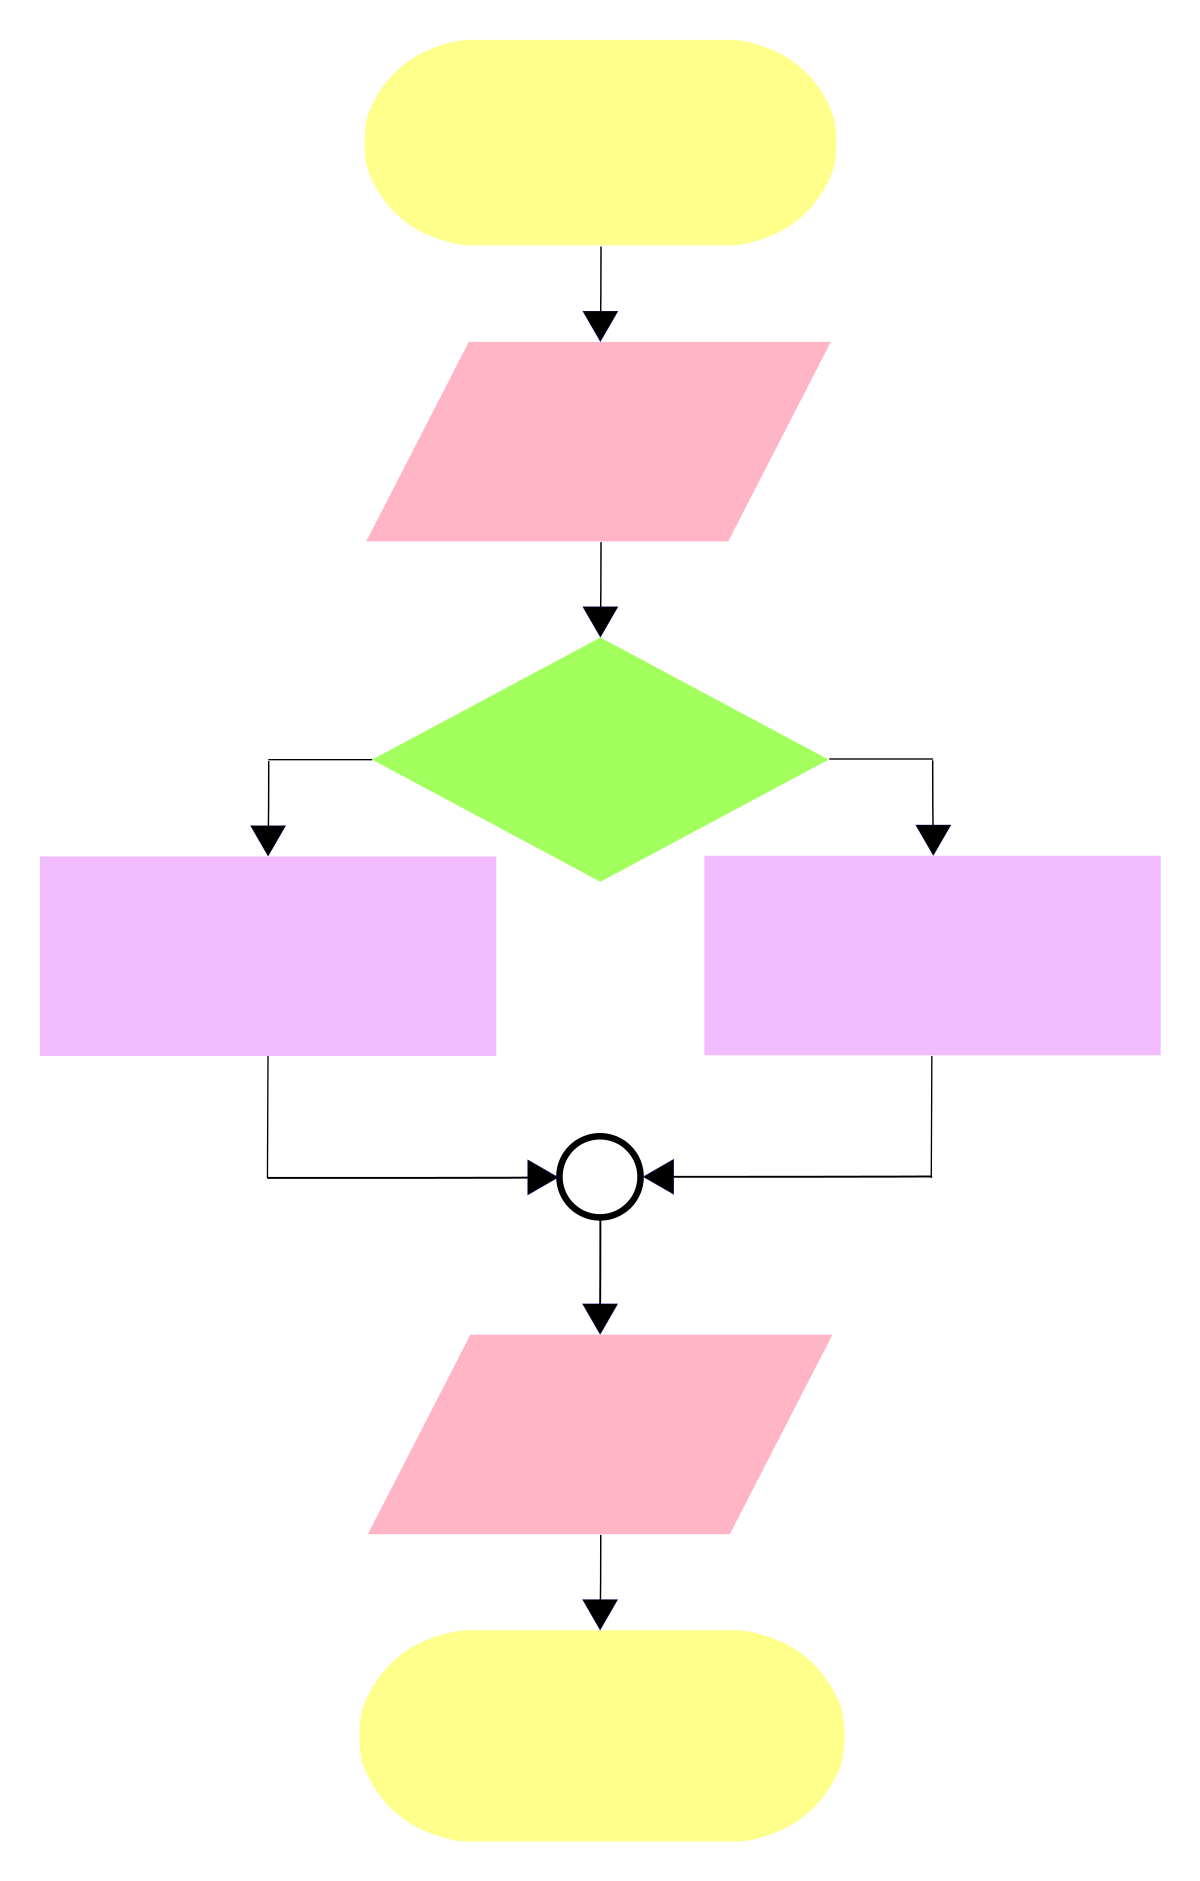
\includegraphics[width=7cm]{./gambar/flowchart.png}
    \caption{Diagram alir penelitian.}
    \label{fig:diagramAlirPenelitian}
\end{figure}


%=====================================================================
\section{Jenis dan Desain Penelitian}
%=====================================================================

...


%=====================================================================
\section{Lokasi dan Waktu Penelitian}
%=====================================================================

...


%=====================================================================
\section{Prosedur Penelitian}
%=====================================================================

%---------------------------------------------------------------------
\subsection{Perangkat Penelitian}
%---------------------------------------------------------------------

%Lorem ipsum.
%\setlist{nolistsep}
%\begin{enumerate}[noitemsep]
%    \item Lorem ipsum.
%    \item ...
%\end{enumerate}


%---------------------------------------------------------------------
\subsection{Langkah Kerja}
%---------------------------------------------------------------------

\vspace{3mm}

\subsubsection{Subsubbagian 1}

%Lorem ipsum.
%\setlist{nolistsep}
%\begin{enumerate}[noitemsep]
%    \item Lorem ipsum.
%    \item ...
%\end{enumerate}

\subsubsection{Subsubbagian 2}

%Lorem ipsum.
%\setlist{nolistsep}
%\begin{enumerate}[noitemsep]
%    \item Lorem ipsum.
%    \item ...
%\end{enumerate}

\subsubsection{Subsubbagian 3}

%Lorem ipsum.
%\setlist{nolistsep}
%\begin{enumerate}[noitemsep]
%    \item Lorem ipsum.
%    \item ...
%\end{enumerate}
    %%%%%%%%%%%%%%%%%%%%%%%%%%%%%%%%%%%%%%%%%%%%%%%%%%%%%%%%%%%%%%%%%%%%%%
%%%%%%%%%%%%%%%%%%%%%%%%%%%%%%%%%%%%%%%%%%%%%%%%%%%%%%%%%%%%%%%%%%%%%%
% BAB METODOLOGI PENELITIAN:
%=====================================================================
\renewcommand{\thechapter}{\Roman{chapter}}
\addtocontents{toc}{\vskip10pt}
\chapter{HASIL DAN PEMBAHASAN}
\renewcommand{\thechapter}{\arabic{chapter}}
%---------------------------------------------------------------------

%=====================================================================
\section{Bagian 1}
%=====================================================================

...
%Lorem ipsum.
%\setlist{nolistsep}
%\begin{enumerate}[noitemsep]
%    \item Lorem ipsum.
%    \item ...
%\end{enumerate}


%---------------------------------------------------------------------
\subsection{Subbagian 1}
%---------------------------------------------------------------------

...
%Lorem ipsum.
%\setlist{nolistsep}
%\begin{enumerate}[noitemsep]
%    \item Lorem ipsum.
%    \item ...
%\end{enumerate}


%---------------------------------------------------------------------
\subsection{Subbagian 2}
%---------------------------------------------------------------------

...
%Lorem ipsum.
%\setlist{nolistsep}
%\begin{enumerate}[noitemsep]
%    \item Lorem ipsum.
%    \item ...
%\end{enumerate}


%=====================================================================
\section{Bagian 2}
%=====================================================================

...
%Lorem ipsum.
%\setlist{nolistsep}
%\begin{enumerate}[noitemsep]
%    \item Lorem ipsum.
%    \item ...
%\end{enumerate}



    %%%%%%%%%%%%%%%%%%%%%%%%%%%%%%%%%%%%%%%%%%%%%%%%%%%%%%%%%%%%%%%%%%%%%%
%%%%%%%%%%%%%%%%%%%%%%%%%%%%%%%%%%%%%%%%%%%%%%%%%%%%%%%%%%%%%%%%%%%%%%
% BAB PENUTUP
%=====================================================================
\renewcommand{\thechapter}{\Roman{chapter}}
\addtocontents{toc}{\vskip10pt}
\chapter{PENUTUP}
\renewcommand{\thechapter}{\arabic{chapter}}
%---------------------------------------------------------------------

%=====================================================================
\section{Kesimpulan}
%=====================================================================

Ini adalah contoh tulisan untuk bagian kesimpulan yang apabila dirincikan dapat dituliskan sebagai berikut:

\begin{enumerate}
    \item Saran 1. 
    \item Saran 2.
    \item Saran 3.
\end{enumerate}

%=====================================================================
\section{Saran}
%=====================================================================
\begin{enumerate}
    \item Kesimpulan 1.
    \item Kesimpulan 2.
\end{enumerate}


    
%---------------------------------------------------------------------
%   DAFTAR PUSTAKA
%---------------------------------------------------------------------

    \addtocontents{toc}{\vskip10pt}
    \renewcommand{\bibname}{DAFTAR PUSTAKA}
    \addcontentsline{toc}{chapter}{DAFTAR PUSTAKA}
    %\bibliographystyle{unsrt} % untuk style dengan nomor
    \bibliographystyle{format-pustaka} % untuk style dengan nama
    \bibliography{pustaka}
    
%---------------------------------------------------------------------
%   APPENDIX
%---------------------------------------------------------------------

    {
    \appendix
    \addtocontents{toc}{\vskip10pt}
    \renewcommand{\chaptername}{LAMPIRAN}
    %%%%%%%%%%%%%%%%%%%%%%%%%%%%%%%%%%%%%%%%%%%%%%%%%%%%%%%%%%%%%%%%%%%%%%
% LAMPIRAN A
%%%%%%%%%%%%%%%%%%%%%%%%%%%%%%%%%%%%%%%%%%%%%%%%%%%%%%%%%%%%%%%%%%%%%%

\chapter{Judul Lampiran}

%---------------------------------------------------------------------
\section{Lampiran}
%---------------------------------------------------------------------

Tuliskan lampiran di sini.

%%%%%%%%%%%%%%%%%%%%%%%%%%%%%%%%%%%%%%%%%%%%%%%%%%%%%%%%%%%%%%%%%%%%%%
    %\input{./halaman-belakang/lampiran/lampiranB}
    }
%---------------------------------------------------------------------
%   BIOGRAFI PENULIS
%---------------------------------------------------------------------

    %%%%%%%%%%%%%%%%%%%%%%%%%%%%%%%%%%%%%%%%%%%%%%%%%%%%%%%%%%%%%%%%%%%%%%
%%%%%%%%%%%%%%%%%%%%%%%%%%%%%%%%%%%%%%%%%%%%%%%%%%%%%%%%%%%%%%%%%%%%%%
% BIOGRAFI PENULIS
%=====================================================================
\renewcommand{\thechapter}{\Roman{chapter}}
\addtocontents{toc}{\vskip10pt}
\chapter*{BIOGRAFI PENULIS}
\renewcommand{\thechapter}{\arabic{chapter}}
%---------------------------------------------------------------------

\begin{wrapfigure}{l}{.35\textwidth}
  \begin{center}
    \vspace{-20pt} % Silahkan disesuaikan apabila space di atas gambar terlalu kecil/besar
    
\includegraphics[width=.30\textwidth]{./gambar/foto.png}
    \vspace{-20pt} % Silahkan disesuaikan apabila space di bawah gambar terlalu kecil/besar
  \end{center}
\end{wrapfigure}

\noindent Biodata singkat mengenai penulis dapat dituliskan pada bagian ini. Gambar diri dari \textit{file} "foto.jpeg" dalam folder  \textbf{gambar} akan ditampilkan di bagian atas kalimat ini. \lipsum[1-2]
 
\vspace{7pt}
\noindent Email: \emailMahasiswa

%======================================================================
    
%=====================================================================
\end{document}
%=====================================================================

%%%%%%%%%%%%%%%%%%%%%%%%%%%%%%%%%%%%%%%%%%%%%%%%%%%%%%%%%%%%%%%%%%%%%%